\documentclass[thesis]{subfiles}

\begin{document}

\chapter{Protokół komunikacji}
\label{chapter:protokol}

Opracowany protokół komunikacji, użyty między serwerem i~klientem, opiera się na~protokole~TCP. Bezpieczeństwo protokołu zapewnia wykorzystanie biblioteki OpenSSL, która implementuje protokół~SSL/TLS. Oba te~elementy, tzn.~opracowany protokół aplikacji oraz~wykorzystana biblioteka OpenSSL, działają w~warstwie aplikacji modelu~\gls{tcpip}, co~przedstawia tabela~\ref{fig:protocol-big-view}.

W~niniejszym rozdziale opisano wszystkie rodzaje pakietów przesyłanych między klientem i~serwerem oraz~sposób i~przyczynę wykorzystania biblioteki OpenSSL w~projekcie.

\begin{table}
\centering
\renewcommand{\arraystretch}{1.3}
\begin{tabular}{l|l|l|l}
	   & Warstwy modelu OSI & Warstwy modelu TCP/IP~(DoD)       & Wykorzystane protokoły \\\hline\hline
	1. & Aplikacji          & \multirow{3}{*}{Aplikacji}        & \multirow{3}{*}{\parbox{3.5cm}{Opracowany \mbox{protokół} + SSL/TLS}} \\\cline{1-2}
	2. & Prezentacji        &                                   & \\\cline{1-2}
	3. & Sesji              &                                   & \\\hline
	4. & Transportowa       & Transportowa                      & TCP \\\hline
	5. & Sieciowa           & Internetu                         & IPv4 \\\hline
	6. & Łącza danych       & \multirow{2}{*}{Dostępu do sieci} & \multirow{2}{*}{Ethernet} \\\cline{1-2}
	7. & Fizyczna           &                                   &
\end{tabular}
\caption{Wykorzystane protokoły sieciowe i~ich umiejscowienie w~modelach OSI~i~TCP/IP~(DoD)}
\label{fig:protocol-big-view}
\end{table}

%------------------------------------------------------------------------------

\section{Rodzaje pakietów}

W~opracowanym protokole występuje kilka typów pakietów, które są~wysyłane między klientem i~serwerem. W~zależności od~etapu i~okoliczności komunikacji, wykorzystywany jest różny typ pakietu. Pakiety są~rozróżnialne między sobą dzięki polu \texttt{TYPE} pakietu, określającym jego rodzaj. Pole \texttt{TYPE} jest jednym z~elementów nagłówka pakietu. Nagłówek pakietu jest wspólny dla~wszystkich rodzajów pakietów. Rysunek~\ref{fig:packet-common} przedstawia schemat pamięci wszystkich rodzajów pakietów.

\newcommand\packetheader{%
	\begin{leftwordgroup}{Nagłówek\\pakietu}%
		\bitbox{4}{VER}%
		\bitbox{12}{FLAGS}%
		\bitbox{16}{TYPE}%
	\end{leftwordgroup}\\
}

\begin{figure}
	\centering
	\begin{bytefield}{32}
		\bitheader{0,3,4,7,8,11,12,15,16,19,20,23,24,27,28,31}\\
		\packetheader
		\begin{leftwordgroup}{Pola zależne od~typu\\pakietu określonego\\przez pole \texttt{TYPE}}
			\wordbox[lrt]{1}{\vdots}\\
			\skippedwords\\
			\wordbox[lrb]{2}{\vdots}
		\end{leftwordgroup}\\
	\end{bytefield}
	\caption{Wspólny schemat pamięci wszystkich pakietów opracowanego protokołu}
	\label{fig:packet-common}
\end{figure}

% Inne propozycje co może zawierać nagłówek (może się przydać, a może nie):
% language, encoding, length, md5

Znaczenie poszczególnych pól nagłówka:\mynobreakpar
\begin{enumerate}
	\item \texttt{VER} (\emph{Protocol Version}, 4~bity) --- Wersja protokołu. Jedyna akceptowalna obecnie wartość to~$1$. Pole to~jest znane z~różnych, powszechnie używanych protokołów i~zostało wprowadzone z~myślą o~ewentualnych przyszłych wersjach protokołu, w~których mogłyby zajść duże zmiany w~układzie pól pakietów.

	Strona połączenia, która otrzyma pakiet z~nieznaną wersją protokołu odpowiada pakietem typu \texttt{PROTO\_FAILURE} z~ustawionym kodem błędu \texttt{UNKNOWN\_PROTO\_VER}.

	\item \texttt{FLAGS} (\emph{Protocol Flags}, 12~bitów) --- Maska bitowa określająca flagi protokołu. Znaczenie flag protokołu zależy od~typu pakietu, czyli od~pola \texttt{TYPE}.

	Strona połączenia, która otrzyma pakiet z~ustawionymi bitami, które nie mają zdefiniowanego znaczenia w~wersji protokołu \texttt{VER}, odpowiadają pakietem \texttt{PROTO\_FAILURE} z~ustawionym kodem błędu~\texttt{UNKNOWN\_FLAG}.
	%	\begin{itemize}
	%		\item $\texttt{0000}_{\texttt{(2)}} = \texttt{0}_{\texttt{(10)}}$ --- Wszystkie flagi wyczyszczone.
	%		\item $\texttt{0001}_{\texttt{(2)}} = \texttt{1}_{\texttt{(10)}}$ --- Wartość na~razie niewykorzystana. (TODO)
	%		\item $\texttt{0010}_{\texttt{(2)}} = \texttt{2}_{\texttt{(10)}}$ --- Wartość na~razie niewykorzystana. (TODO)
	%		\item $\texttt{0100}_{\texttt{(2)}} = \texttt{3}_{\texttt{(10)}}$ --- Wartość na~razie niewykorzystana. (TODO)
	%		\item $\texttt{1000}_{\texttt{(2)}} = \texttt{4}_{\texttt{(10)}}$ --- Wartość na~razie niewykorzystana. (TODO)
	%	\end{itemize}

	\item \texttt{TYPE} (\emph{Packet Type}, 16~bitów) --- Typ pakietu określający jaką rolę pakiet odgrywa w~komunikacji. Dopuszczalne wartości odpowiadające kolejnym liczbom naturalnym\footnote{Przyjmujemy konwencję, że~$0$ należy do liczb naturalnych ($0\in\mathbb{N}$).}:
	\begin{itemize}
		\item \texttt{UPGRADE\_REQUEST (0x00)} --- Żądanie aktualizacji wysłane przez klienta do~serwera~(patrz rozdział~\ref{full-upgrade-request}).
		\item \texttt{UPGRADE\_RESPONSE (0x01)} --- Odpowiedź serwera na~żądanie aktualizacji \texttt{UPGRADE\_REQUEST} wysłane przez klienta~(patrz rozdział~\ref{full-upgrade-response}).
		\item \texttt{UPGRADE\_STATUS (0x02)} --- Status powodzenia aktualizacji klienta po~otrzymaniu pakietu \texttt{UPGRADE\_RESPONSE}~(patrz rozdział~\ref{full-upgrade-status}).
		\item \texttt{PROTO\_FAILURE (0x03)} --- Błąd połączenia~(patrz rozdział~\ref{proto-failure}).
	\end{itemize}

	Strona połączenia, która otrzyma pakiet z~niezdefiniowaną w~protokole w~wersji \texttt{VER}, wartością pola \texttt{TYPE}, odpowiada pakietem \texttt{PROTO\_FAILURE} z~ustawionym kodem błędu \texttt{UNKNOWN\_PACKET\_TYPE}.
\end{enumerate}

W~dalszej części rozdziału zostaną omówione rodzaje przesyłanych pakietów, wykorzystywanych w~opracowanym protokole m.in.~do~zarządzania oprogramowaniem klientów i~obsługą sytuacji awaryjnych.

%---------------------------------------

\subsection{Żądanie aktualizacji klienta}
\label{full-upgrade-request}

Pakiet z~żądaniem aktualizacji oprogramowania jest przesyłany przez klienta do~serwera i~oznacza chęć dostosowania oprogramowania klienta do~wzorca serwera. Taki rodzaj pakietu jest symbolicznie oznaczany w~kodzie programu nazwą \texttt{UPGRADE\_REQUEST}~(patrz~rys.~\ref{fig:packet-full-upgrade-request}). Nazwa ta, jak również nazwy innych pakietów przesyłanych w~ramach opracowanego protokołu, są~zdefiniowane jako typ wyliczeniowy~\texttt{enum~packet\_t} w~jednym z~plików nagłówkowych współdzielonych przez program serwera i~klienta. Typ pakietu jest przesyłany w~nagłówku każdego pakietu przesyłanego między klientem i~serwerem.

\begin{figure}[h]
	\centering
	\begin{bytefield}{32}
		\bitheader{0,3,4,7,8,11,12,15,16,19,20,23,24,27,28,31}\\
		\packetheader
		\bitbox{16}{CONFIG\_SET} & \bitbox{8}{COMPR\_TYPE} & \bitbox{8}{PKG\_MGR}\\
		\wordbox{1}{LAST\_UPGRADE\_TIME}\\
	\end{bytefield}
	\caption{Schemat pamięci pakietu typu~\texttt{UPGRADE\_REQUEST}}
	\label{fig:packet-full-upgrade-request}
\end{figure}

Serwer może mieć wiele wzorców oprogramowania dla~różnych klientów, dlatego klient przesyła do~serwera numer~wybranego zestawu konfiguracji. Numery konfiguracji odpowiadają różnym zapotrzebowaniom konfiguracji komputerów. Przykładowo, laboratorium komputerowe przeznaczone na~potrzebny nauki systemów CAD/CAM może mieć inny zestaw oprogramowania od~tego używanego w~salach w~bibliotece, co~jest odzwierciedlone przez przypisanie różnych numerów oprogramowania dla~komputerów w~tych salach. Maksymalna ilość różnych zestawów konfiguracji jest zdeterminowana przez 16-sto bitowy rozmiar pola i~wynosi~$2^{16}=65536$.

Aktualizacja oprogramowania klienta może się wiązać z~przesłaniem znacznej ilości danych~(rzędu setek megabajtów lub kilku gigabajtów), szczególnie gdy klient synchronizuje się z~serwerem po~raz pierwszy lub synchronizacja nie była uruchamiana od~dłuższego czasu. Istnieje więc potrzeba zastosowania bezstratnej kompresji przesyłanego oprogramowania. Pole \texttt{COMPR\_TYPE} pakietu typu \texttt{UPGRADE\_REQUEST}, umożliwia ustawienie jednej z~kilku predefiniowanych rodzajów kompresji.

Znaczenie poszczególnych pól dla pakietu typu \texttt{UPGRADE\_REQUEST}:\mynobreakpar
\begin{enumerate}
	\item \texttt{CONFIG\_SET} (\emph{Configuration Setting Number}, 16~bitów) --- Numer konfiguracji z~zakresu $[0;2^{16}-1]\cap\mathbb{Z}$, któremu odpowiada zestaw oprogramowania przeznaczony dla~klienta. Numery konfiguracji służą do~rozróżniania zapotrzebowania komputerów na~oprogramowanie. Przykładowo komputery w~pracowniach komputerowych i~w~bibliotece mogą mieć przydzielone różne numery \texttt{CONFIG\_SET}, ponieważ komputery te~wymagają różnej konfiguracji i~oprogramowania.
	\item \texttt{COMPR\_TYPE} (\emph{Compression Type}, 8~bitów) --- Sposób kompresji jaki zostanie użyty do~spakowania pakietów, które zostaną przesłane do~klienta. Szerokość pola pozwala na~zdefiniowanie maksymalnie~$2^8=256$ rodzajów kompresji. W~pierwszej wersji protokołu istnieje 6~rodzajów akceptowanych wartości, które odpowiadają kolejnym liczbom naturalnym:
		\begin{itemize}
			\item \texttt{NO\_COMPRESSION (0x00)} --- brak kompresji,
			\item \texttt{TAR\_GZ\_COMPRESSION (0x01)} --- kompresja do~archiwum \path{*.tar.gz} komendą \texttt{tar~czf},
			\item \texttt{TAR\_BZ2\_COMPRESSION (0x02)} --- kompresja do~archiwum \path{*.tar.bz2} komendą \texttt{tar~cjf},
			\item \texttt{TAR\_XZ\_COMPRESSION (0x03)} --- kompresja do~archiwum \path{*.tar.xz} komendą \texttt{tar~cJf},
			\item \texttt{RAR\_COMPRESSION (0x04)} --- kompresja do~archiwum \path{*.rar} komendą \texttt{rar~a},
			\item \texttt{ZIP\_COMPRESSION (0x05)} --- kompresja do~archiwum \path{*.zip} komendą \texttt{zip}.
		\end{itemize}
	Jeśli serwer otrzyma pakiet z~nieznanym sposobem kompresji odpowiada pakietem typu \texttt{PROTO\_FAILURE} z~ustawionym kodem błędu \texttt{UNKNOWN\_COMPR\_TYPE}.
	\item \texttt{PKG\_MGR} (\emph{Package Manager}, 8~bitów) --- Rodzaj menadżera pakietów używanego przez klienta. W~zależności od~wartości tego pola, klient otrzyma paczki oprogramowania przeznaczone dla~różnych menadżerów pakietów. Ośmiobitowa szerokość pola umożliwia rozszerzenie wsparcia dla~nowych menadżerów pakietów w~kolejnych wersjach protokołu. Dopuszczalne wartości tego pola odpowiadają kolejnym liczbom naturalnym:
		\begin{itemize}
			\item \texttt{DPKG\_PKG\_MGR (0x00)} --- Paczki oprogramowania \texttt{*.deb} przeznaczone dla~systemów korzystających z~menadżera pakietów \texttt{dpkg}\footnote{W~praktyce wykorzystywane są~menadżery pakietów \texttt{apt-get} i~\texttt{aptitude}, które ,,rozumieją'' zależności pomiędzy pakietami i~korzystają z~niskopoziomowego~\texttt{dpkg}.}, wykorzystanego w~takich dystrybucjach \gls{gnulinux} jak np.~\emph{Debian} i~systemy bazujące na~nim, np.~\emph{Ubuntu}, \emph{Knoppix}, \emph{Linux~Mint} czy~\emph{Damn Small Linux~(DSL)},
			\item \texttt{TAR\_XZ\_PKG\_MGR (0x01)} --- Paczki oprogramowania \texttt{*.pkg.tar.xz} przeznaczone dla~systemów korzystających z~menadżera pakietów \texttt{pacman}, wykorzystanego w~systemie \emph{Arch~Linux}.
		\end{itemize}
	\item \texttt{LAST\_UPGRADE\_TIME} (\emph{Last Upgrade Time}, 32~bity) --- Czas ostatniej synchronizacji oprogramowania klienta z~serwerem. Na~podstawie tego pola serwer wie które pakiety i~elementy konfiguracji muszą zostać przesłane do~klienta, a~które zostały już przesłane. Jeśli pole to~jest wyzerowane, to~serwer prześle klientowi wszystkie pakiety jakie są~przewidziane dla~danego \texttt{CONFIG\_SET}. W~szczególności jest to~użyteczne, gdy klient przesyła pakiet typu \texttt{UPGRADE\_REQUEST} po~raz pierwszy.
\end{enumerate}

Algorytm działania sewera po~otrzymaniu pakietu typu~\texttt{UPGRADE\_REQUEST}:\mynobreakpar
\begin{enumerate}
	\item Sprawdź czy~pakiet przesłany przez klienta jest poprawnie sformatowany, tzn.~czy ma~oczekiwaną długość i~czy wszystkie pola pakietu są~akceptowalne. W~szczególności sprawdź czy~menadżer pakietów przesłany w~polu~\texttt{PKG\_MGR} jest wspierany przez serwer. Jeśli pakiet nie jest sformatowany poprawnie, prześlij pakiet \texttt{PROTO\_FAILURE} z~kodem błędu odpowiadającym przyczynie niepowodzenia.
	\item\label{create-file} Zapisz w~katalogu \path{/var/run} plik tekstowy zawierający informację o~rozpoczęciu komunikacji z klientem, który zgłosił żądanie typu~\texttt{UPGRADE\_REQUEST}. Krok ten ma za~zadanie zagwarantować transakcyjność operacji, tzn. że w~przypadku awaryjnego wyjścia z~programu serwera, serwer po ponownym uruchomieniu będzie miał szansę poinformować administratora w~swoich logach o~niepowodzeniu aktualizacji klienta oraz podjąć kroki mające na~celu przywrócenie integralności stanu serwera.
	\item Na~podstawie pola \texttt{LAST\_UPGRADE\_TIME} sprawdź czy~klient wymaga aktualizacji. Jeśli klient jest już zaktualizowany, to~prześlij pakiet \texttt{UPGRADE\_RESPONSE} (patrz rozdział~\ref{full-upgrade-response}) z~wyzerowanym polem \texttt{LENGTH} i~zakończ połączenie. W~przeciwnym razie przejdź do~kolejnego punktu algorytmu.
	\item Odczytaj pole \texttt{CONFIG\_SET} otrzymanego pakietu i~na jego podstawie ustal który plik konfiguracyjny odczytać. Plik ten definiuje zestaw oprogramowania dla klienta. W~przypadku odczytania nieobsługiwanej wartości \texttt{CONFIG\_SET}, odeślij pakiet \texttt{PROTO\_FAILURE} z~ustawionym kodem błędu \texttt{UNKNOWN\_CONFIG\_SET}.
	\item Odczytaj powyższy plik konfiguracyjny. W~przypadku gdy plik ten nie istnieje, nie daje się odczytać, ma nieoczekiwany format lub z~dowolnego innego powodu, uniemożliwiającego dalsze działanie na jego podstawie, prześlij do~klienta pakiet typu \texttt{PROTO\_FAILURE} z~kodem błędu \texttt{SERVER\_INTERNAL\_ERR}. W~przeciwnym przypadku, na~podstawie pliku konfiguracyjnego i~pola \texttt{LAST\_UPGRADE\_TIME} otrzymanego pakietu, ustal listę pakietów, które należy przesłać do~klienta.
	\item Na~podstawie przygotowanej listy pakietów, pobierz z~cache'a pakiety dla~klienta, a~tych których nie ma w~cache'u, pobierz z~internetu ze~źródła zdefiniowanego w~pliku konfiguracyjnym serwera. Pobrane pliki zapisz w~cache'u, usuwając najdłużej nieużywane pliki z~cache'a jeśli jest osiągnięto limit wykorzystania cache'a. \textbf{Uwaga:} wykonanie tego kroku przez serwer może być czasochłonne ze~względu na~konieczność pobrania pakietów z~internetu. W~przypadku przerwania pobierania dowolnego pakietu z~internetu, serwer przesyła klientowi pakiet typu \texttt{PROTO\_FAILURE} z~kodem błędu \texttt{SERVER\_INTERNAL\_ERR}. W~przypadku zerwania połączenia z~klientem, serwer kontynuuje pobieranie wszystkich pakietów, dzięki czemu klient szybko otrzyma\footnote{Pod warunkiem, że~cache nie zostanie wyczyszczony.} aktualizację oprogramowania po~ponownym wysłaniu pakietu typu \texttt{UPGRADE\_REQUEST}.
	\item Utwórz z~wszystkich pakietów przeznaczonych dla~klienta archiwum typu określonego polem \texttt{COMPR\_TYPE} pakietu. Jeśli kompresja nie powiedzie się z~dowolnego powodu, wyślij pakiet typu \texttt{PROTO\_FAILURE} z~kodem błędu \texttt{SERVER\_INTERNAL\_ERR}.
	\item Wyślij archiwum z~pakietami do~klienta. Archiwum to~nie jest podpisywane cyfrowo przez serwer, ponieważ przesłanie archiwum odbywa się~w~ramach sesji~SSL/TLS, na~początku której klient uwierzytelnia serwer sprawdzając jego cyfrowy certyfikat.
	\item Oczekuj na~raport o~powodzeniu instalacji. Odnotuj w~logach raport od~klienta. \textbf{Uwaga:} oczekiwanie może być czasochłonne, dlatego serwer czeka na potwierdzenie przez pewien czas. (TODO: szczegółowy opis jak to obsłużyć).
	\item Zakończ połączenie i~skasuj plik utworzony w~kroku~\ref{create-file}.
\end{enumerate}

%---------------------------------------

\subsection{Odpowiedź na żądanie aktualizacji klienta}
\label{full-upgrade-response}

Po~otrzymaniu przez serwer pakietu typu \texttt{UPGRADE\_REQUEST}, serwer analizuje czy klient jest już zaktualizowany, a~jeśli nie, to co~powinien otrzymać od~serwera w~odpowiedzi. Odpowiedź serwera ma~typ pakietu \texttt{UPGRADE\_RESPONSE} i~składa się z~następujących pól:

\begin{itemize}
	\item  \texttt{LENGTH} (\emph{Total Length}, 64~bity) --- Długość pola \texttt{DATA} w~bajtach. Akceptowalne wartości z~przedziału $[0;2^{64}]$. Wartość~$0$ oznacza, że~klient jest już zaktualizowany i~nie potrzebuje dokonywać żadnych zmian, aby~dostosować się do~wzorca serwera.
	\item \texttt{DATA} (\emph{Upgrade Data}, \texttt{LENGTH}~bitów) --- Archiwum żądanego przez klienta typu (por.~\ref{full-upgrade-request}) z~pakietami i~konfiguracją do~zainstalowania na~kliencie. Rozmiar tego pola wynosi~\texttt{LENGTH} bajtów.
\end{itemize}

\begin{figure}[h]
	\centering
	\begin{bytefield}{32}
		\bitheader{0,3,4,7,8,11,12,15,16,19,20,23,24,27,28,31}\\
		\packetheader
		\wordbox{2}{LENGTH}\\
		\wordbox[lrt]{1}{DATA}\\
		\skippedwords\\
		\wordbox[lrb]{2}{\vdots}
	\end{bytefield}
	\caption{Schemat pamięci pakietu typu~\texttt{UPGRADE\_RESPONSE}}
	\label{fig:packet-full-upgrade-response}
\end{figure}

%---------------------------------------

\subsection{Status powodzenia instalacji oprogramowania}
\label{full-upgrade-status}

Klient po~otrzymaniu od~serwera oprogramowania w~pakiecie typu \texttt{UPGRADE\_RESPONSE}, instaluje je, a~następnie informuje serwer o~powodzeniu lub~niepowodzeniu aktualizacji wysyłając do~serwera pakiet \texttt{UPGRADE\_STATUS} z~ustawionym kodem statusu~\texttt{STATUS\_CODE}~(patrz rys.~\ref{fig:packet-full-upgrade-status}).

\begin{figure}[h]
	\centering
	\begin{bytefield}{32}
		\bitheader{0,3,4,7,8,11,12,15,16,19,20,23,24,27,28,31}\\
		\packetheader
		\wordbox{1}{STATUS\_CODE}
	\end{bytefield}
	\caption{Schemat pamięci pakietu typu~\texttt{UPGRADE\_STATUS}}
	\label{fig:packet-full-upgrade-status}
\end{figure}

%---------------------------------------

\subsection{Błąd połączenia}
\label{proto-failure}

Istnieje wiele możliwych sytuacji, w~których dalsza komunikacja między serwerem i~klientem jest bezcelowa i~powinna zostać zakończona. Przykładami takich sytuacji jest~np.~błędnie sformatowany przychodzący pakiet lub~nieobsługiwana wersja protokołu. W~takich przypadkach strona połączenia, która wykryje taką sytuację, powinna zakomunikować drugiej stronie, że~kończy połączenie z~powodu określonego kodem błędu. Pakiety przeznaczone do~tego celu to~pakiety typu \texttt{PROTO\_FAILURE}. Budowa takiego pakietu została przedstawiona na~rysunku~\ref{fig:packet-protocol-failure}, a~dopuszczalne typy błędów zostały opisane w~tabeli~\ref{fig:packet-protocol-failure-desc}.

\begin{figure}[h]
	\centering
	\begin{bytefield}{32}
		\bitheader{0,3,4,7,8,11,12,15,16,19,20,23,24,27,28,31}\\
		\packetheader
		\bitbox{16}{ERR\_CODE} & \bitbox{16}{\color{lightgray}\rule{\width}{\height}}\\
	\end{bytefield}
	\caption{Schemat pamięci pakietu typu~\texttt{PROTO\_FAILURE}}
	\label{fig:packet-protocol-failure}
\end{figure}

\begin{table}
\centering
\renewcommand{\arraystretch}{1.3}
\begin{tabular}{l|p{1.5cm}|p{8.5cm}}
	Kod błędu                      & Numer błędu   & Znaczenie kodu błędu\\\hline\hline
	\texttt{UNKNOWN\_PROTO\_VER}   & \texttt{0x00} & Pole \texttt{VER} określa nieobsługiwaną wersję protokołu.\\\hline
	\texttt{UNKNOWN\_FLAG}         & \texttt{0x01} & Pole \texttt{FLAGS} ma~ustawione bity, które nie są rozpoznawane w~tej wersji protokołu.\\\hline
	\texttt{UNKNOWN\_PKG\_MGR}     & \texttt{0x02} & Pole \texttt{PKG\_MGR} określa nieobsługiwany menadżer pakietów.\\\hline
	\texttt{UNKNOWN\_COMPR\_TYPE}  & \texttt{0x03} & Pole \texttt{COMPR\_TYPE} określa nieznany zestaw oprogramowania.\\\hline
	\texttt{UNKNOWN\_CONFIG\_SET}  & \texttt{0x04} & Pole \texttt{CONFIG\_SET} określa nieznany zestaw oprogramowania.\\\hline
	\texttt{UNKNOWN\_PACKET\_TYPE} & \texttt{0x05} & Pole \texttt{TYPE} określa nieznany typ pakietu.\\\hline
	\texttt{MALFORMED\_PACKET}     & \texttt{0x06} & Pakiet jest niepoprawnie sformatowany z~innego powodu niż powyższe.\\\hline
	\texttt{SERVER\_INTERNAL\_ERR} & \texttt{0x07} & Wystąpił błąd po~stronie serwera.\\\hline
	\texttt{CLIENT\_INTERNAL\_ERR} & \texttt{0x08} & Wystąpił błąd po~stronie klienta.
\end{tabular}
\caption{Kody błędów dla~pakietu typu \texttt{PROTO\_FAILURE} i~ich znaczenie}
\label{fig:packet-protocol-failure-desc}
\end{table}

%------------------------------------------------------------------------------

\section{Bezpieczeństwo protokołu}
\label{sec:security}

Uwzględnienie bezpieczeństwa protokołu jest krytyczne dla~powodzenia projektu protokołu, szczególnie takiego, który umożliwia serwerowi na~zarządzanie konfiguracją dziesiątek, setek lub tysięcy klientów. Zaniedbanie bezpieczeństwa protokołu lub~jego wadliwa implementacja, umożliwiłaby atakującemu system, na~przejęcie kontroli nad~wszystkimi klientami, np.~przez przesłanie klientom złośliwych aktualizacji oprogramowania lub~konfiguracji.

Umożliwienie przejęcia kontroli nad wszystkimi klientami byłoby prawdopodobnie najgorszym z~możliwych scenariuszy zarówno dla użytkowników jak i~administratora atakowanej sieci, jednak niedbała implementacja protokołu mogłaby umożliwiać również wiele innych rodzajów ataków, np. \emph{replay attack} i~\emph{man in the middle~(MITM)}. W~celu uniknięcia podatności protokołu na~wymienione i~inne, popularne rodzaje ataków, należy zagwarantować bezpieczeństwo protokołu co~najmniej pod względem:
\begin{enumerate}
\item uwierzytelnienia co~najmniej serwera,
\item poufności komunikacji,
\item integralności komunikacji.
\end{enumerate}
W~celu maksymalnego zaostrzenia rygorów bezpieczeństwa protokołu, do powyższych własności można dodać również inne, w~szczególności, własność \emph{\glslink{pfs}{Perfect Forward Secrecy~(PFS)}} (patrz rozdział~\ref{sec:pfs}).

W~kolejnych podrozdziałach zostaną opisane metody, które zostały wykorzystane do~zapewnienia poszczególnych elementów, składających się na~bezpieczeństwo protokołu. Wszystkie opisane dalej algorytmy i~metody kryptograficzne zostały wykorzystane przez niniejszy projekt przez wykorzystanie popularnej, otwartoźródłowej biblioteki kryptograficznej~\gls{openssl}, implementującej protokół kryptograficzny~\gls{ssl/tls}.

%---------------------------------------

\subsection{SSL/TLS}
\label{sec:ssl-tls}

Protokół \gls{ssl/tls} jest bardzo elastyczny pod względem doboru algorytmów i~metod kryptograficznych. Elastyczność objawia się nie tylko możliwością skonfigurowania konkretnych algorytmów, które posłużą do~zapewnienia uwierzytelnienia, poufności, integralności komunikacji i~ustalenia klucza sesji, ale również możliwością zdefiniowania za pomocą słów kluczowych, zbioru algorytmów spośród których serwer i~klient, podczas negocjacji w~ramach \emph{handshake'u} sesji \gls{ssl/tls}, wybierają jeden, najsilniejszy z~tych, które wspierają.

Przykładowo, jeśli celem jest dopuszczenie do~użytku wyłącznie zestawów metod kryptograficznych używających algorytmu \glslink{dh}{Diffiego-Hellmana} do~wymiany klucza, a~do szyfrowania szyfru blokowego~\gls{aes}, to filtr będzie miał postać napisu \texttt{DH+AES @STRENGTH}. Słowo kluczowe \texttt{@STRENGTH} służy do posortowania wynikowych zestawów metod kryptograficznych nierosnąco (a~nie ściśle malejąco) względem bezpieczeństwa.

Aby przekonać się jakie algorytmy zostaną zwrócone dla danego filtru, nie~trzeba korzystać z~API biblioteki \gls{openssl}. Wystarczy nam do~tego konsola, co~prezentuje listing~\ref{openssl-console-filter}.\\

\begin{lstlisting}[numbers=none,language=bash,caption={Wynik filtrowania zestawów algorytmów w~konsoli za~pomocą \gls{openssl}},label=openssl-console-filter]
$ openssl ciphers -v 'DH+AES @STRENGTH'
AES256-GCM-SHA384   TLSv1.2 Kx=RSA  Au=RSA  Enc=AESGCM(256)  Mac=AEAD
AES256-SHA256       TLSv1.2 Kx=RSA  Au=RSA  Enc=AES(256)     Mac=SHA256
AES256-SHA          SSLv3 Kx=RSA    Au=RSA  Enc=AES(256)     Mac=SHA1
AES128-GCM-SHA256   TLSv1.2 Kx=RSA  Au=RSA  Enc=AESGCM(128)  Mac=AEAD
AES128-SHA256       TLSv1.2 Kx=RSA  Au=RSA  Enc=AES(128)     Mac=SHA256
AES128-SHA          SSLv3 Kx=RSA    Au=RSA  Enc=AES(128)     Mac=SHA1
\end{lstlisting}

Filtr złożony ze~słów kluczowych, wykorzystany w~implementacji projektu zarówno dla serwera, jak i~klienta, został przedstawiony na listingu~\ref{openssl-filter}. Filtr ten jest bardzo restrykcyjny, tak, aby zapewnić~\gls{pfs}. Wykrzyknik w filtrze pełni rolę operatora logicznego~\texttt{not}.\\

\begin{lstlisting}[numbers=none,caption={Filtr \gls{openssl} dla algorytmów użytych w~projekcie},label=openssl-filter]
kEECDH+ECDSA kEECDH kEDH +SHA !aNULL !eNULL !LOW !3DES !MD5 !EXP !DSS !PSK !SRP !kECDH !CAMELLIA !IDEA !RC4 !SEED @STRENGTH
\end{lstlisting}

Pełny opis słów kluczowych można znaleźć w~dokumentacji \gls{openssl} oraz w~darmowej, regularnie aktualizowanej elektronicznej książce\footnote{Jest ona częścią większej książki pt.~,,Bulletproof SSL and TLS"~(ISBN:~978-1907117046). Projekt \gls{openssl} ma~raczej opinię słabo udokumentowanego, dlatego te~książki mają spore znaczenie praktyczne.} pt.~,,OpenSSL Cookbook'' autorstwa Ivana Ristić'a, polecanej na~oficjalnej stronie internetowej projektu~\gls{openssl}~\cite{openssl-cookbook-suites}.

%---------------------------------------

\subsection{Uwierzytelnienie}

Uwierzytelnienie serwera przez klienta jest krytyczne dla~bezpieczeństwa protokołu. Gdyby nie ono, to~atakujący mógłby podawać się za~serwer i~przesłać klientowi dowolną konfigurację i~oprogramowanie. Gdyby komunikacja była szyfrowana, ale nieuwierzytelniona, to atakujący mógłby również podjąć próby ataku \emph{replay attack}. W~celu uniknięcia tego problemu wykorzystano certyfikat X.509 dla~serwera~\cite{wiki:x509}.

Wygenerowanie takiego certyfikatu wymaga podpisania przez centrum certyfikacji~(\gls{ca})~\cite{wiki:ca}. Ze~względu na~brak potrzeby posiadania w~trakcie implementacji certyfikatu podpisanego przez uznane \gls{ca}, a~także ze względu na~względnie duże koszty finansowe i~czasowe z~tym związane, w czasie implementacji wykorzystano certyfikat podpisany przez siebie~(ang.~\emph{self-signed certificate}). Konfiguracja klienta pozwala w~trybie \texttt{debug} zaufać takiemu certyfikatowi. Oczywiście, w~przypadku wdrożenia projektu, należałoby postarać się o~certyfikat podpisany przez uznany~\gls{ca}.

Wygenerowanie i~podpisanie certyfikatu zostało wykonane z~użyciem \gls{openssl}. Listing~\ref{openssl-gencert} przedstawia jak wygenerować klucze publiczny i~prywatny \gls{rsa} o~długości 4096~bitów, a~następnie, jak wykorzystać klucz prywatny do~wygenerowania żądania podpisania certyfikatu (ang.~\emph{Certificate signing request}) i~na jego podstawie podpisać certyfikat~X.509~\cite{openssl-cookbook,wiki:csr}.

\begin{lstlisting}[numbers=none,caption={Wygenerowanie i~podpisanie certyfikatu X.509},label=openssl-gencert]
$ openssl genrsa -aes256 -out rsa_aes256_4096.key 4096
$ openssl req -new -key rsa_aes256_4096.key -out request.csr
$ openssl req -new -config request.cnf -key fd.key -out request.csr
$ openssl x509 -req -days 365 -in request.csr -signkey rsa_aes256_4096.key -out certificate.pem
\end{lstlisting}

Przykładowa zawartość pliku \path{request.cnf}, który służy do~konfiguracji żądania podpisania certyfikatu przedstawia listing~\ref{openssl-request-config}.

\begin{lstlisting}[numbers=none,caption={Plik z~konfiguracją certyfikatu X.509},label=openssl-request-config]
[req]
default_bits       = 4096
default_keyfile    = rsa_aes256_4096.key
prompt             = no
distinguished_name = dn
req_extensions     = ext
input_password     = minipw

[dn]
CN                 = Patryk
OU                 = MiNI
emailAddress       = patryk.beza@gmail.com
O                  = PW
L                  = Warsaw
ST                 = Masovian
C                  = PL

[ext]
subjectAltName     = DNS:www.mini.pw.edu.pl,DNS:*.mini.pw.edu.pl
\end{lstlisting}

Aby sprawdzić czy~certyfikat jest przez nas zaufany, wystarczy wydać komendę:
\begin{lstlisting}[numbers=none]
$ openssl verify -verbose certificate.pem
\end{lstlisting}

%---------------------------------------

\subsection{Poufność}

Poufność komunikacji nie jest tak krytyczna jak uwierzytelnienie serwera, jednak jest również istotna, ponieważ atakujący podsłuchujący komunikację między serwerem i~klientami, mógłby się~wiele dowiedzieć o~wersjach i~konfiguracji oprogramowania klientów. Dzięki zdobytej wiedzy, atakujący mógłby przeanalizować np.~czy oprogramowanie klientów jest przestarzałe i~podatne na~ataki, czy konfiguracja oprogramowania pozwala na~wykorzystanie luk bezpieczeństwa.

Komunikacja między serwerem i~klientem jest szyfrowana symetrycznym, blokowym szyfrem \gls{aes} z~kluczem 256-bitowym~(preferowane podczas negocjacji) lub~128-bitowym. Dla~obu długości klucza możliwe jest działanie w~trybie~GCM\footnote{\emph{Galois/Counter Mode}.}~(preferowane) lub~domyślnym.

%---------------------------------------

\subsection{Integralność}

Integralność komunikacji jest konieczna, aby zapobiec atakom typu \emph{man in the middle}, polegającym na~modyfikacji komunikacji między serwerem i~klientem, niezależnie od~tego czy jest ona~szyfrowana czy nie.

Algorytm używany do~sprawdzania integralności wiadomości jest negocjowany tak jak algorytmy używane do~zapewnienia uwierzytelnienia, szyfrowania i~ustalenia wspólnego klucza dla symetrycznego algorytmu szyfrującego komunikację (patrz rozdział~\ref{sec:ssl-tls}). Możliwe algorytmy to: \emph{AEAD}\footnote{Ściśle rzecz biorąc tryb AEAD~(ang.~\emph{Authenticated Encryption with Associated Data}) jest klasą wiązania bloków zaszyfrowanych w~blokowym algorytmie szyfrującym (ang.~\emph{Block cipher mode of operation}. \gls{aes} pracujący w trybie GCM należy do~tej klasy, dzięki czemu integralność jest zapewniana ,,przy okazji" szyfrowania komunikacji.}, \emph{SHA384}, \emph{SHA256} i~\emph{SHA1}.

%---------------------------------------

\subsection{Perfect Forward Secrecy}
\label{sec:pfs}

Własność \emph{\glslink{pfs}{Perfect Forward Secrecy}~(PFS)} umożliwia zachowanie poufności komunikacji nawet jeśli atakujący zapisał całą zaszyfrowaną komunikację między serwerem i~klientem, a~po~jakimś czasie uzyskał klucze prywatne obu stron komunikacji. Własność ta~wiąże się ze sposobem ustalenia sesyjnego klucza dla~symetrycznego szyfru zapewniającego poufność komunikacji (takiego jak np.~\gls{aes}).

W~uproszczeniu problem polega na tym, że~w~przypadku wykorzystania~\gls{rsa} do~ustalenia klucza sesyjnego dla~symetrycznego algorytmu szyfrującego, strona~A komunikacji, używa klucza publicznego strony~B do~zaszyfrowania losowego klucza sesyjnego\footnote{W~rzeczywistości \emph{Pre-Master Key}, z~którego dopiero jest wyliczany ostateczny klucz sesyjny.}~i wysyła go~do~B. Po~skompromitowaniu klucza prywatnego strony~B, atakujący może odczytać całą komunikację między stronami A~i~B, deszyfrując najpierw klucz sesyjny, a~następnie całą komunikację między serwerem i~klientem.

\gls{pfs} radzi sobie z~tym problemem rezygnując z~przesyłania zaszyfrowanego klucza sesyjnego, wprowadzając zamiast tego efemeryczny algorytm \glslink{dh}{Diffiego-Hellmana} w~postaci klasycznej~(\glslink{dh}{EDH})~i krzywoeliptycznej~(ECDHE)~\cite{mimuw-ssl-w04,openssl-cookbook-suites}. Efemeryczny algorytm \glslink{dh}{Diffiego-Hellmana} różni się od~nieefemerycznego tym, że~w~efemerycznej wersji algorytmu parametry algorytmu nie~są stałe, tzn. np.~nie są zapisane w~certyfikacie. Wersja krzywoliniowa co do~pomysłu nie różni się istotnie od~wersji klasycznej, tylko działa na krzywych eliptycznych. Wersja krzywoeliptyczna charakteryzuje się~lepszą wydajnością na~większości procesorów ze~względu na~fakt, że~do zapewnienia takiego samego poziomu bezpieczeństwa jakie gwarantuje~\gls{rsa} z~kluczem o~długości 3072~bitów, potrzeba krzywoeliptycznego odpowiednika o~długości 256~bitów.

Poniżej został przedstawiony schemat przebiegu klasycznego algorytmu \glslink{dh}{Diffiego-Hellmana}.

\begin{enumerate}
\item A i~B uzgadniają skończoną, cykliczną grupę~$G$ rzędu~$p$, gdzie $p$ jest liczbą pierwszą i~generator $g$ tej grupy. Atakujący może znać~$g$ oraz~$p$.
\item A wybiera tajną liczbę całkowitą $1 \leq a < n$ i~wysyła do~B liczbę $A=g^a \pmod{p}$.
\item B wybiera tajną liczbę całkowitą $1 \leq b < n$ i~wysyła do~A liczbę $B=g^b \pmod{p}$.
\item A oblicza $s=B^a \pmod{p}$.
\item B oblicza $s=A^b \pmod{p}$.
\item A i~B współdzielą tajną liczbę~$s$.
\end{enumerate}

Podsłuchujący atakujący, aby~poznać liczbę $s$, musiałby rozwiązać tzw.~problem Diffiego-Hellmana, który jest problemem równie trudnym w~sensie teorii złożoności, jak problem algorytmu dyskretnego. Liczby $a$ i~$b$ są~przed wysłaniem podpisywane kluczem prywatnym w celu uniknięcia ataku~\emph{man in the middle}.

Ilustracja~\ref{fig:dh} obrazowo przedstawia w~jaki sposób działa algorytm \glslink{dh}{Diffiego-Hellmana}.

\begin{figure}
	\centering
	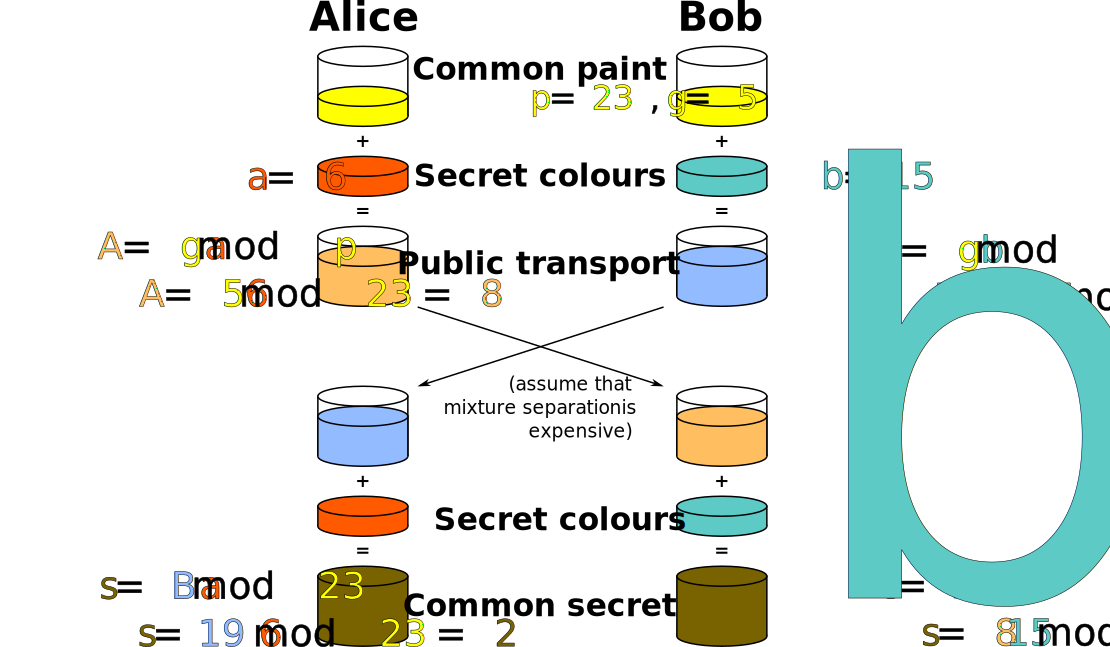
\includegraphics[width=\textwidth]{img/Diffie-Hellman_Key_Exchange_desc}
	\caption{Zobrazowanie działania algorytmu Diffiego-Hellmana (źródło: Wikipedia)}
	\label{fig:dh}
\end{figure}

%---------------------------------------

\subsection{Zestawy kryptograficzne}

W~praktyce, podczas testów, w~czasie których nawiązywano połączenie \gls{ssl/tls} pomiędzy klientem i~serwerem uruchamianym na~systemie z~zainstalowanym \gls{openssl} w~wersji \texttt{1.0.2h}, strony połączenia zawsze negocjowały zestaw algorytmów \texttt{ECDHE-RSA-AES256-GCM-SHA384}, który oznacza użycie najnowszego dostępnej wersji protokołu~\glslink{ssl/tls}{TLS}, tj.~protokołu~TLSv1.2, zapewniającego:
\begin{enumerate}
\item Poufność przez wykorzystanie \gls{aes} pracującym w trybie GCM z~kluczem o~długości 256~bitów,
\item Ustalenie klucza sesyjnego dla~\gls{aes} przez~wykorzystanie efemerycznej wersji algorytmu \glslink{dh}{Diffiego-Hellmana} w~wersji dla~krzywych eliptycznych~(ECDH),
\item Uwierzytelnienie przez wykorzystanie podpisu cyfrowego z~wykorzystaniem~\gls{rsa},
\item Integralność gwarantowaną przez działanie \gls{aes} w~trybie~GCM. SHA384~w~nazwie wynegocjonowanego zestawu oznacza uczycie funkcji haszującej SHA384 podczas fazy \emph{handshake} i~do rozszerzenia dzielonego sekretu uzyskanego podczas ustalenia klucza~sesyjnego do~klucza symetrycznego dla~\gls{aes}~\cite{stack:openssl-sha-gcm}.
\end{enumerate}

\end{document}
